\documentclass[12pt,a4paper]{article}

\usepackage{float}
\restylefloat{figure}
\usepackage{hyperref}
\usepackage{graphicx}
\usepackage{gensymb}
\usepackage[title]{appendix}
\usepackage[dotinlabels]{titletoc}
\usepackage[nottoc,numbib]{tocbibind}
\usepackage{mathtools}
\usepackage[margin=0.5in]{geometry}
\renewcommand{\thefootnote}{\arabic{footnote}}

\newcommand*\wrapletters[1]{\wr@pletters#1\@nil}
\def\wr@pletters#1#2\@nil{#1\allowbreak\if&#2&\else\wr@pletters#2\@nil\fi}

\usepackage{enumitem}
\setenumerate{itemsep=0pt}

\pagenumbering{Roman}

\title{MEng Final Year Project Plan}
\author{Chris Cummins}

\begin{document}
\maketitle

\begin{abstract}
\noindent
This document contains a proposal and plan to develop a Protein Isoelectric
Point Database as a final year project, under the supervision of Professor Ian
Nabney and based on research undertaken by Dr. Darren Flower and members of
Aston University's Life and Health Sciences department.
\end{abstract}
\newpage

\tableofcontents
\listoffigures
\listoftables

\newpage
\pagenumbering{arabic}


\section{INTRODUCTION \hrulefill}

The purpose of the project is to make an intuitive and powerful bioinformatics
search engine which provides online access to a large dataset of protein
isoelectric points which has been compiled by Aston University researchers and
students over the course of several years.

\subsection{Background}
Bioinformatics is a multidisciplinary field which uses computational methods to
aid in biological research by creating systems for storing, organising and
analysing complex biological data. Within this field there are many online
databases categorising biological information at the molecular level, and one
such purpose of these is for storing the functional and physical properties of
proteins. Currently, no such database exists for one of the most widely-used,
important, and useful properties of proteins: the isoelectric point (pI). An
isoelectric point is the acidity (pH) at which a molecule carries no net charge;
below the isoelectric point, proteins have a net positive charge, above it a net
negative charge. Additionally, proteins are at their lowest solubility at their
isoelectric point, and this makes the isoelectric point a vitally important
property when both characterising and purifying proteins.

The dataset which has been compiled is a collection of entries stored as a
non-relational table, and for each entry it records the name of the protein, its
identity, origin, experimental conditions, its isoelectric point, and other
pertinent data. There are also links to a heterogeneous collection of databases
containing associated data, such as amino acid sequence, function, etc. A
website that warehouses this data and offers a robust and adaptable GUI for
searching, viewing and downloading results would greatly increase the
accessibility of the dataset.

\subsection{Objectives}

\begin{enumerate}
\item To build a free (as in freedom) web application for searching and viewing
  protein isoelectric points.
\item To produce a bioinformatics tool with real world value for future
  research.
\item The application should provide intuitive but powerful searching
  facilities.
\item The application should provide a convenient means for a certified user to
  edit and upload additional data.
\item The application should present information in a usable and efficient form.
\item Users should be allowed to download generated results for offline use.
\item Adequate security precautions should be taken to minimise the risk of data
  being sabotaged or stolen.
\item The implementation should use a clean model view controller architecture.
\item Comprehensive test coverage of the API and common use cases should be
  automated.
\item The application should be scalable for much larger datasets.
\end{enumerate}

\subsection{Deliverables}
Two primary deliverables can be derived from the project objectives:

\begin{enumerate}
\item An updatable relational database warehousing the provided dataset.
\item A web-accessible GUI with searching and downloading functionality.
\end{enumerate}

Additionally, two further deliverables can be derived from the same requirements
document as secondary features:

\begin{enumerate}
\item A web-accessible GUI to support editing and uploading new data.
\item Support for NCBI BLAST protein sequence matching (1).
\end{enumerate}
%TODO: ref

\subsection{Required Resources}
The deliverable product for this product is a website that offers a publicly
available service. To this end, there are three required resources:

\begin{enumerate}
\item A server which can be host the website and process and respond to requests
  from clients.
\item A public IP address which this server can be assigned to for external
  access.
\item A domain name which will resolve to this IP address.
\end{enumerate}

Additional stipulations for the requirements are that the server should use a
GNU/Linux operating system so as to support most common webserver stacks, and
that it should be a dedicated physical machine with root access so as to allow
for more involved configuration and testing. Assuming that the University can
supply the webserver and access to one of its IP addresses, the budget for the
project need only cover the cost of domain registration, which is very cheap
(less than £20 per year).

\subsection{Required Technologies}
There are an almost immeasurable number of web technologies that offer the
functionality required to implement this project. From a time-management
perspective, one of the main priorities for the work undertaken in the first
term is to research these existing technologies, and to gain a better
understanding of the strengths of each in order to select an appropriate choice
for the implementation of the final product. Figure 1 shows the process by which
these choices are made, starting off with the highest-level decision (the choice
of paradigms: whether it be a client-server model, a distributed network
application, the format for data transmission etc.) and increasing in
granularity down to the lowest-level choice of individual frameworks and
libraries. Each decision is not immutable, and previous decisions may be
re-evaluated over time in an iterative fashion. This is to encourage
implementation work to begin at an early stage in order to produce a functioning
prototype, without the need to have performed a depth first analysis of every
possible technology which could be used. Work on the implementation can begin
once the programming language(s) have been decided upon, so it is important to
reach a decision upon this as early into TP1 as is possible, although this
decision is free to change over the course of the project, providing there is a
realistic justification for this change and adequate time to re-implement any
existing functionality.

\begin{figure}[H]
\centering
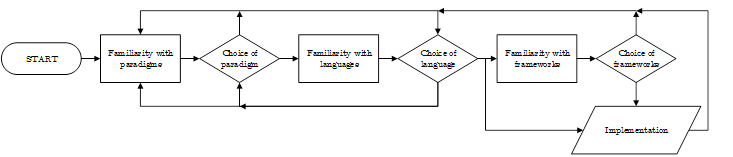
\includegraphics{assets/flow-tech-choices.png}
\caption{A diagrammatic view of the process of adopting technologies}
\label{fig:flow-tech-choices}
\end{figure}

\subsection{Required Skills}
This technically ambitious project will require the adoption of a number of new
skillsets, a brief overview of which is included below:

\subsubsection{Project management}

\paragraph{Single-developer project management} including good communication
with clients and stakeholders, selecting an appropriate software development
process, setting realistic deadlines and goals, and tracking the progress of a
long term development project.

\paragraph{Working with a mature codebase} this includes proper version control
and use of a sane branching model, and documenting decisions and all source code
throughout the duration of development.

\paragraph{Maintenance and tooling} developing a software product with long-term
usability as a primary goal, as well as appropriate documentation to allow other
developers to administrate the website.

\paragraph{Software quality} appropriate use of issue trackers and bug ticketing
to track the lifecycle of implementation bugs and regressions, and adopting a
meaningful release cycle and version numbering scheme.

\subsubsection{Back-end development}

\paragraph{Relational data modelling and database design} designing and
formalising database schemas, and providing advanced querying functionality.

\paragraph{Computing with large datasets} appropriately using existing tools and
software patterns for working with large persistent data models.

\paragraph{Performance optimising} server-side optimisations to enable high
performance serving of web pages such as caching, and successful cache
invalidation techniques for the webserver and database.

\paragraph{Designing secure web applications} using formal and established
methods to ensure data integrity of critical biological research data.

\subsubsection{Front-end development}

\paragraph{User interface design} working with clients to design accessible and
easy-to-user GUIs, including appropriate use of Human Computer Interaction
techniques and user testing.

\paragraph{Responsive website design} correctly using HTML5 and CSS3 features to
allow for site accessibility from a wide range of different devices.

\paragraph{Client-side scripting} using mobile code such as JavaScript to enrich
user interfaces using technologies such as AJAX and dynamic content generation
and control.

\section{INITIAL RESEARCH \hrulefill}

The purpose of the initial project research phase is to enable early
identification of risks, design decisions, and other factors which will
contribute to the creation of the project plan.

\subsection{Analysis of the Dataset}

In order to determine the technical scope of the project it is necessary to
analyse the dataset which the web service will house. The dataset was supplied
by Dr. Flower in the form of a Microsoft Excel spreadsheet consisting of a
single table with 5,773 unique rows over 22 columns. In order to develop a
relational model for this data, each of the 22 unique columns can be considered
as a set of attributes A1,A2,…,A22 and combined to form a relational schema R
(Figure 2 shows this schema with attribute names taken from the spreadsheet
column headings), with the spreadsheet values forming an instance of this
relation r(R) in which each row can be considered a set of tuples where t' =
{t'(A1),t'(A2),…,t'(A22)} ϵ r(R).

\begin{figure}[H]
\centering
\begin{quote}
\textit{R = \{Origin, EC, Protein, Alternative name(s), Source, Organ and/or
  Subcellular locaction, M.W, No., M.W2, No. of Iso-enzymes, pI maximum value,
  pI Min Value, pI Max Value, pI value of major component, pI, Temperature (oC),
  Method, Valid sequence(s) available, UniportKB/ Swiss-Prot/ Protein sequence,
  Species Taxonomy, Full text, Abstract only, Pubmed, Notes\}}
\end{quote}
\caption{A formal relation schema with named attributes}
\label{fig:formal-schema-names-attributes}
\end{figure}

Each tuple represents a single recording of experimentally-derived data, which
lists the origin of the record (such as a research paper, or academic journal),
and 21 attributes which describe the properties of the protein, the experimental
result and the method used to derive it, and links to relevant online
resources. Figure 3 shows a breakdown of the different origins for all of the
records. In order to aid in the design of the database which will be used to
store this dataset, a dataset analysis tool was developed which parses the
dataset file and extracts and derives key information about its properties, and
this information can be used to help determine the best method to use when
storing this data.

\begin{figure}[H]
\centering
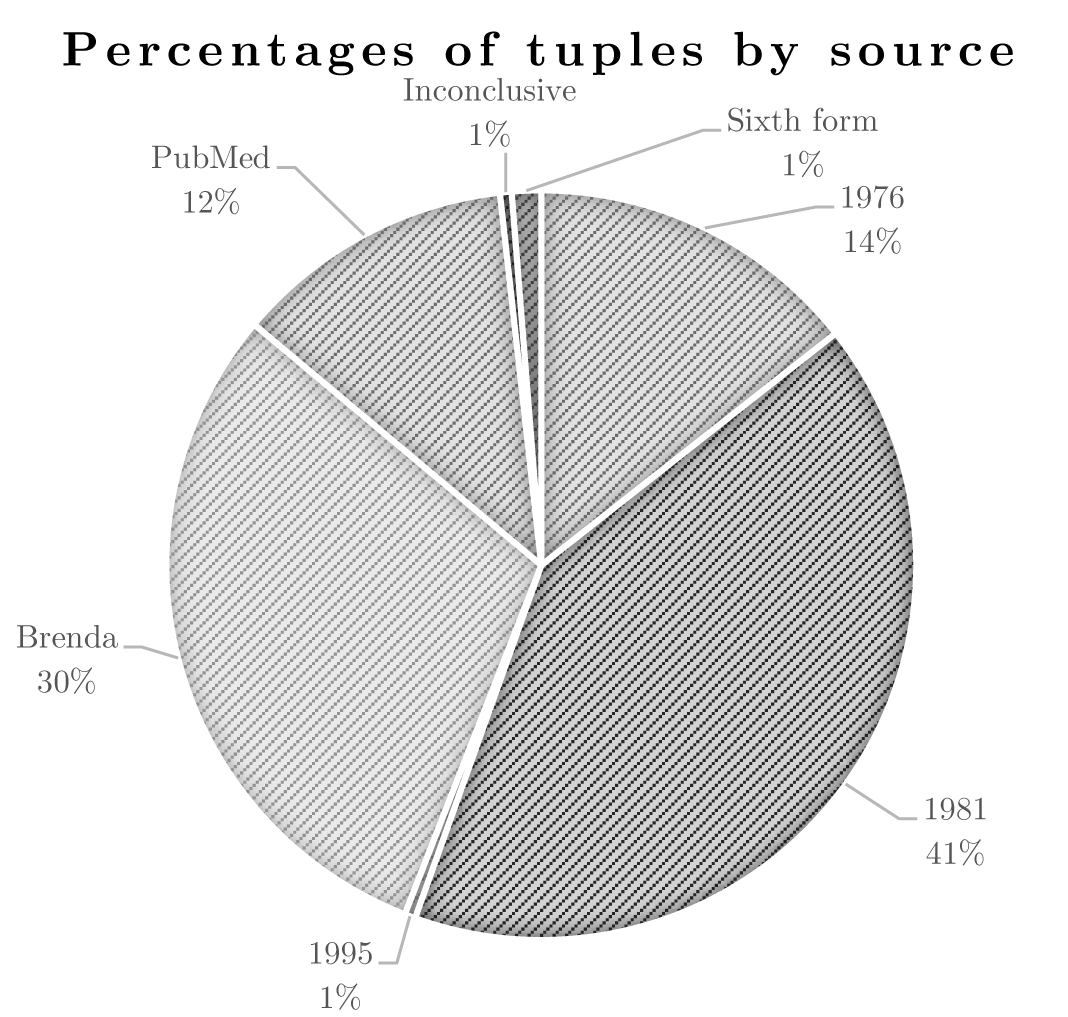
\includegraphics{assets/chart-dataset-origin.png}
\caption{A breakdown of the tuple origins within the dataset}
\label{fig:chart-dataset-origin}
\end{figure}

\newpage
\begin{figure}[H]
\centering
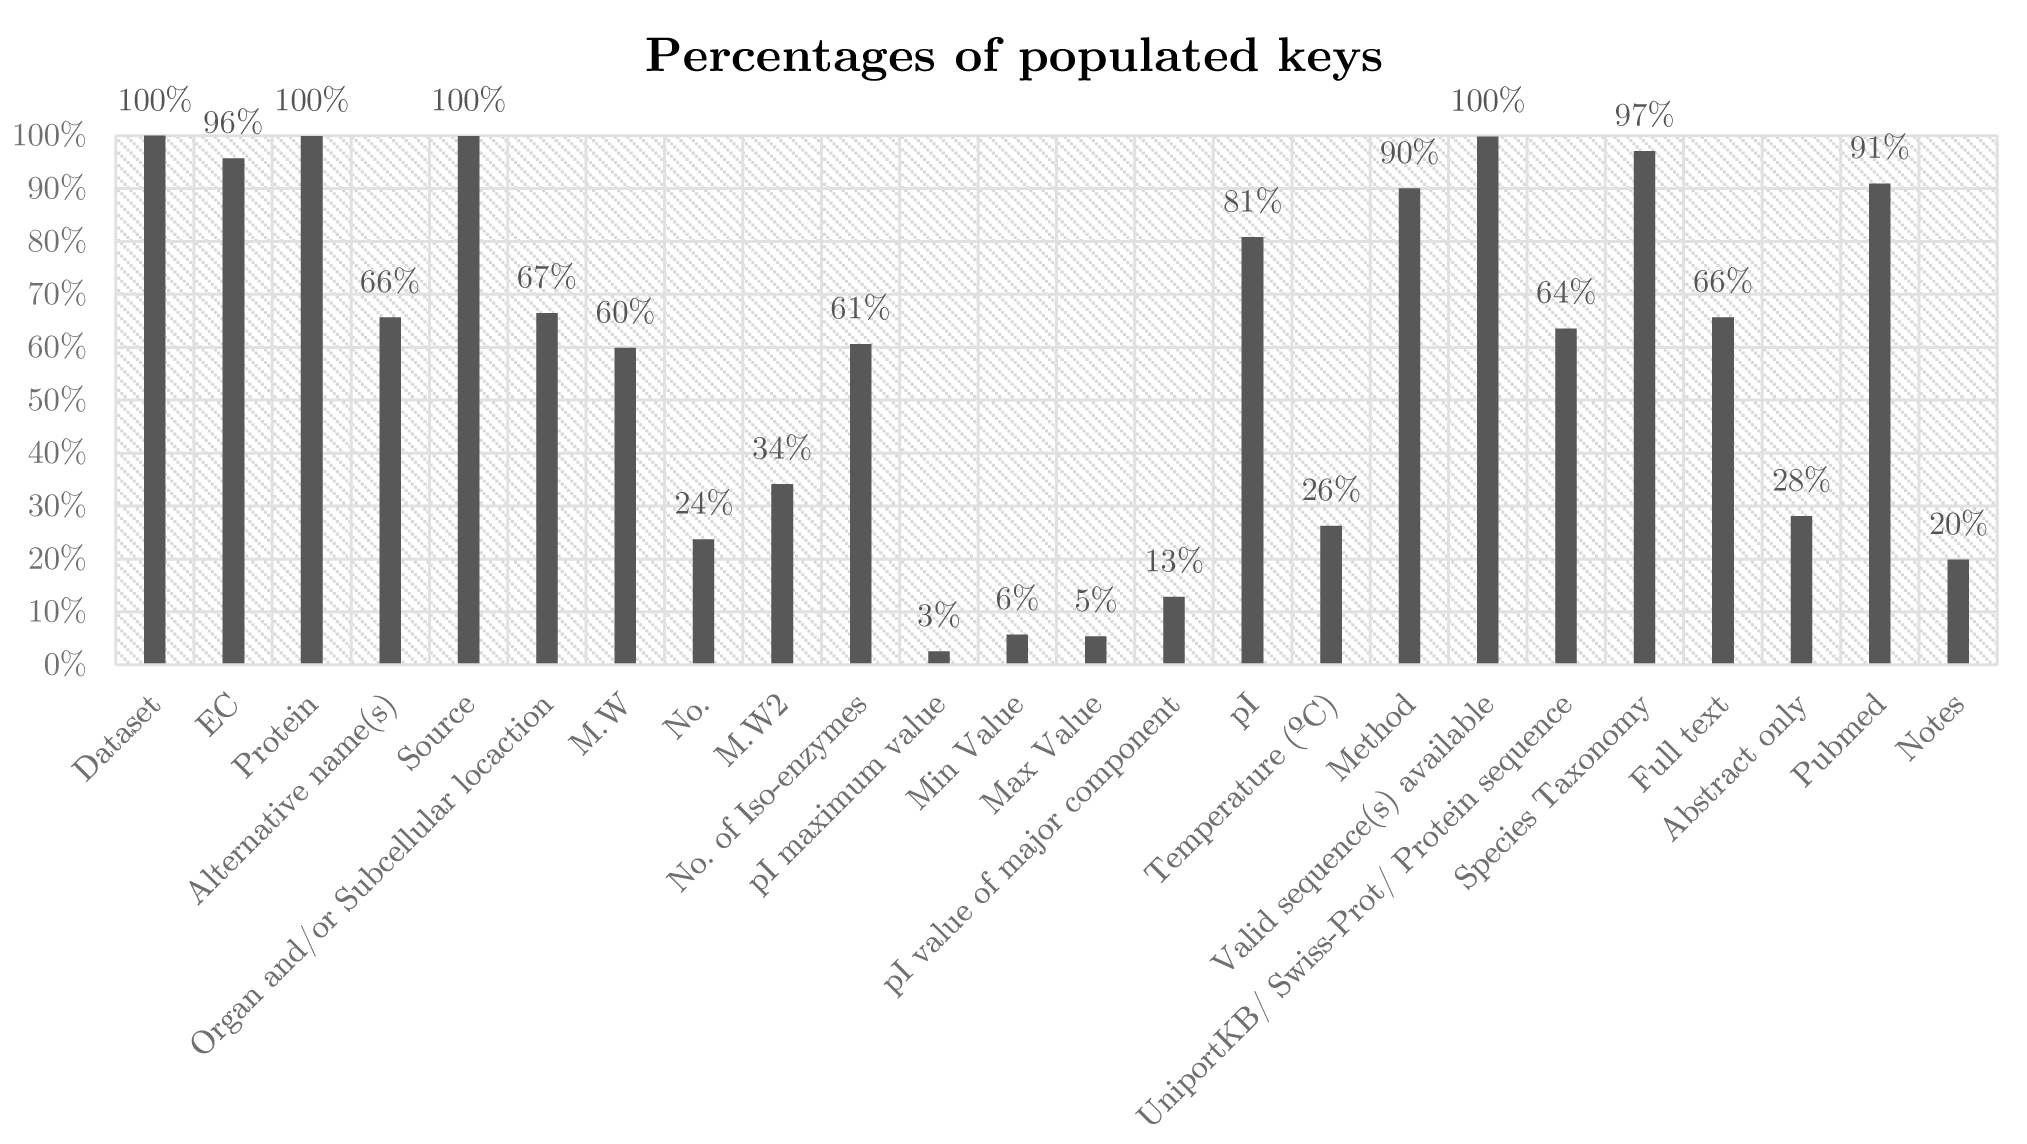
\includegraphics{assets/chart-dataset-populated.png}
\caption{The number of populated keys for each tuple within the dataset}
\label{fig:chart-dataset-populated}
\end{figure}

This early dataset analysis highlighted a number of properties which will
greatly influence the design of the database backend. Chiefly, that the dataset
contains a large number of duplicate keys, and for each tuple, many of the keys
may not be given. This information will have a great influence on the design of
the database; for example, the low percentage of unique values for many of the
records in the dataset indicate that a 3NF normalisation pattern could be used
to gain maximum size efficiency of the stored database (2), and so time should
be allocated in project plan to allow for database design decisions to be
investigated and tested.
% TODO: ref

\begin{figure}[H]
\centering
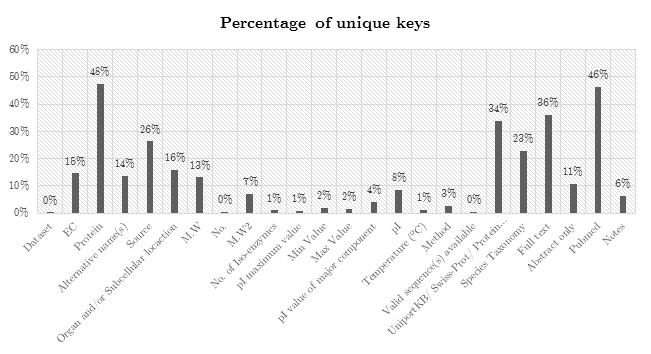
\includegraphics{assets/chart-dataset-unique.png}
\caption{The number of unique keys for each tuple within the dataset}
\label{fig:chart-dataset-unique}
\end{figure}

\newpage
\subsection{Related Bioinformatics Databases}
In addition to gaining a greater understanding of the provided dataset, a
selection of relevant existing websites and databases were examined, in order to
help analyse the strengths and weaknesses of each. As previously stated,
biological databases of protein properties abound, and Dr. Flower's
bioinformatics research has led to the creation of three such databases:
AntiJen, DSD, and PPD:

\paragraph{AntiJen} a kinetic, therm odynam ic and cellular database
(3). AntiJen is a database containing quantitative binding data for
peptides. The database houses over 24,000 entries from published experimentally
determined data, and offers keyword searching of this dataset, with results
being returned in a tabular format.
%TODO: reg

\paragraph{DSD} A database of dehydrogenase stereospecificities (4). DSD offers
a similar set of features as AntiJen but for a different dataset. In addition to
keyword searching, the website supports viewing data by selecting from
categories, and additionally offers BLAST searching, which is a feature that
will incorporated into this project.

\paragraph{PPD} Protein pKa Database (5). PPD offers data lookup by either
BLAST search or a detailed search page which allows the user to select from a
given set of criteria, such as protein name, experimental method, and amino acid
name.

In each of the websites, a large dataset of very specific biological data is
hosted on a website which offers a service for members of the public to query
certain aspects of it and return results. In each case, it is only possible to
return a reduced subset of the data, with no ability for users to download the
entire set in one go; the idea being that users should be allowed to answer
specific queries they may have, but not to idly download the entire dataset
which may be the result of many years of researcher's work. From a technical
standpoint, the websites appear lacking in some areas such as user interface
design, where their rather dated aesthetic and design leads to a rather poor
user experience. Of course this has no bearing on the usefulness of the service
and data offered by the websites, but a greater level of ease of use and control
over the format in which search results are displayed could lead to a more
engaging experience for the user, as well as allowing them to attain the data
they need in a more efficient manner.

\subsection{Previous Final Year Project Analysis}

In addition to the existing public bioinformatics databases which Dr. Flower
assisted in creating, students from previous years have attempted to develop a
similar project to this one. Chief among these was an earlier implementation of
a protein isoelectric point database, created by former student Mohammad
Abdullah. The project used an older and reduced-size version of the current
dataset, and used a MySQL database to store the data, with a PHP back-end to
query the tables and generate static HTML webpages which can be served over an
Apache webserver. A technical review of the implementation revealed a number of
things that could be improved upon – largely that the codebase is a somewhat
impenetrable mixture of PHP with inline HTML, with no distinction between the
application logic and presentation tier, and the querying mechanism is quite
primitive, with little ability to perform advanced searching within the
dataset. Appendix B (page 17) contains a UML diagram of the database schema
used, which highlights the small number of tables used, with few relational
links between records leading to a simplistic searching mechanism.

\newpage
\section{RISK ASSESSMENT \hrulefill}

Table 1 lists some of the potential project risks that were identified during
the initial research phase which could influence the success of the project and
its ability to meet the objectives and deliverables. For each risk, the
probability of it occurring and impact it would have on the project have been
assigned a value between 1 and 5 to indicate their magnitude.

\begin{table}[H]
\centering
\begin{tabular}{ | l | l | l || c | c | }
\hline
Risk & Description & Category & Probability & Impact\\
\hline
R1  & Design is not intuitive                           & Design       & 2 & 3\\
R2  & Project involves use of new technical skills      & Development  & 5 & 5\\
R3  & High Level of technical complexity                & Development  & 5 & 3\\
R4  & Complex deployment of production website          & Development  & 5 & 4\\
R5  & Project milestones not clearly defined            & Planning     & 1 & 1\\
R6  & System requirements not adequately identified     & Requirements & 2 & 5\\
R7  & Change in project requirements during development & Requirements & 1 & 5\\
R8  & Changes in dataset format during development      & Resources    & 2 & 5\\
R9  & Unable to obtain required resources               & Resources    & 1 & 1\\
R10 & Users not committed to the project                & Users        & 2 & 4\\
R11 & Lack of cooperation from users                    & Users        & 1 & 4\\
R12 & Users with negative attitudes toward the project  & Users        & 1 & 2\\
\hline
\end{tabular}
\caption{A list of potential project risks and their severity}
\label{tab:risk-assessment}
\end{table}

\subsection{Mitigation Strategies}

For each of the risks discovered in the assessment, mitigation strategies have
been defined which provide techniques to avoid or minimise the threat of each
risk.

\paragraph{Design is not intuitive} the key to mitigation of this risk is in frequent and
effective user testing and an understanding of typical and common use-cases for
the product.

\paragraph{Project involves use of new technical skills} in order to prevent this risk
from having a serious impact on the project, it will be necessary to begin
studying and reading about the technologies that will be used at a very early
stage in the project, long before the start of the implementation.

\paragraph{High Level of technical complexity} avoiding this risk will involve ensuring
that the scope of the project remains technically feasible, and that the
software architecture is abstracted into small enough units that it is easier to
focus on each one separately, as well as keeping small iterative development
cycles and adequate test coverage to prevent regressions when implementing new
functionality.

\paragraph{Complex deployment of production website} a website with independent
data and application logic components can result in an intricate deployment
process. This is a common problem in the development of complex web application,
where development and production environments must be synchronised and
differences between debugging and releases builds must be accounted for. In
order to mitigate this risk, a suite of tools to configure, build and deploy the
website should be developed at an early stage, allowing for fast deployment of
public releases.

\paragraph{Project milestones not clearly defined} a thoroughly described and well
thought out project plan will help to prevent scheduling issues and delays in
development that would arise from this risk.

\paragraph{System requirements not adequately identified} a comprehensive specification
of the finished product before implementation begins will help to mitigate this
risk.

\paragraph{Change in project requirements during development} an agile approach towards
accommodating for changes in the requirements should be used so as to keep the
time between user feedback sessions and input from stakeholders low.

\paragraph{Changes in dataset form at during development} it is not possible to entirely
avoid this risk due its nature and the dependence on third parties, but steps
can be taken to prevent any delays that this would cause, chiefly, a well
abstracted data parsing component which can be switched and modified if
necessary to accommodate for a new dataset format.

\paragraph{Unable to obtain required resources} since the project does not require many
resources, it is important to acquire these as early on in the development
process as possible, and alternative resources should be planned for, such as
local test servers.

\paragraph{Users not committed to the project, lack of cooperation from users,
  and users with negative attitudes toward the project} the useful of the
finished project will depend largely on ensuring that the needs of the users are
considered the primary goals of the design. Violating this principle may cause
disillusionment from the people who are volunteering their time to assist in the
project.

\section{DEVELOPMENT PROCESS \hrulefill}

The software development process used for this project is based the Open Unified
Process (OpenUP), a part of the Eclipse Process Framework (6). The reasoning
behind this choice is that, as a Rational Unified Process derivative, OpenUP
offers an open source process framework which is targeted at agile development
in small teams and provides a number of development phases and activities which
can be used when designing the project plan (Figure 6).

\begin{figure}[H]
\centering
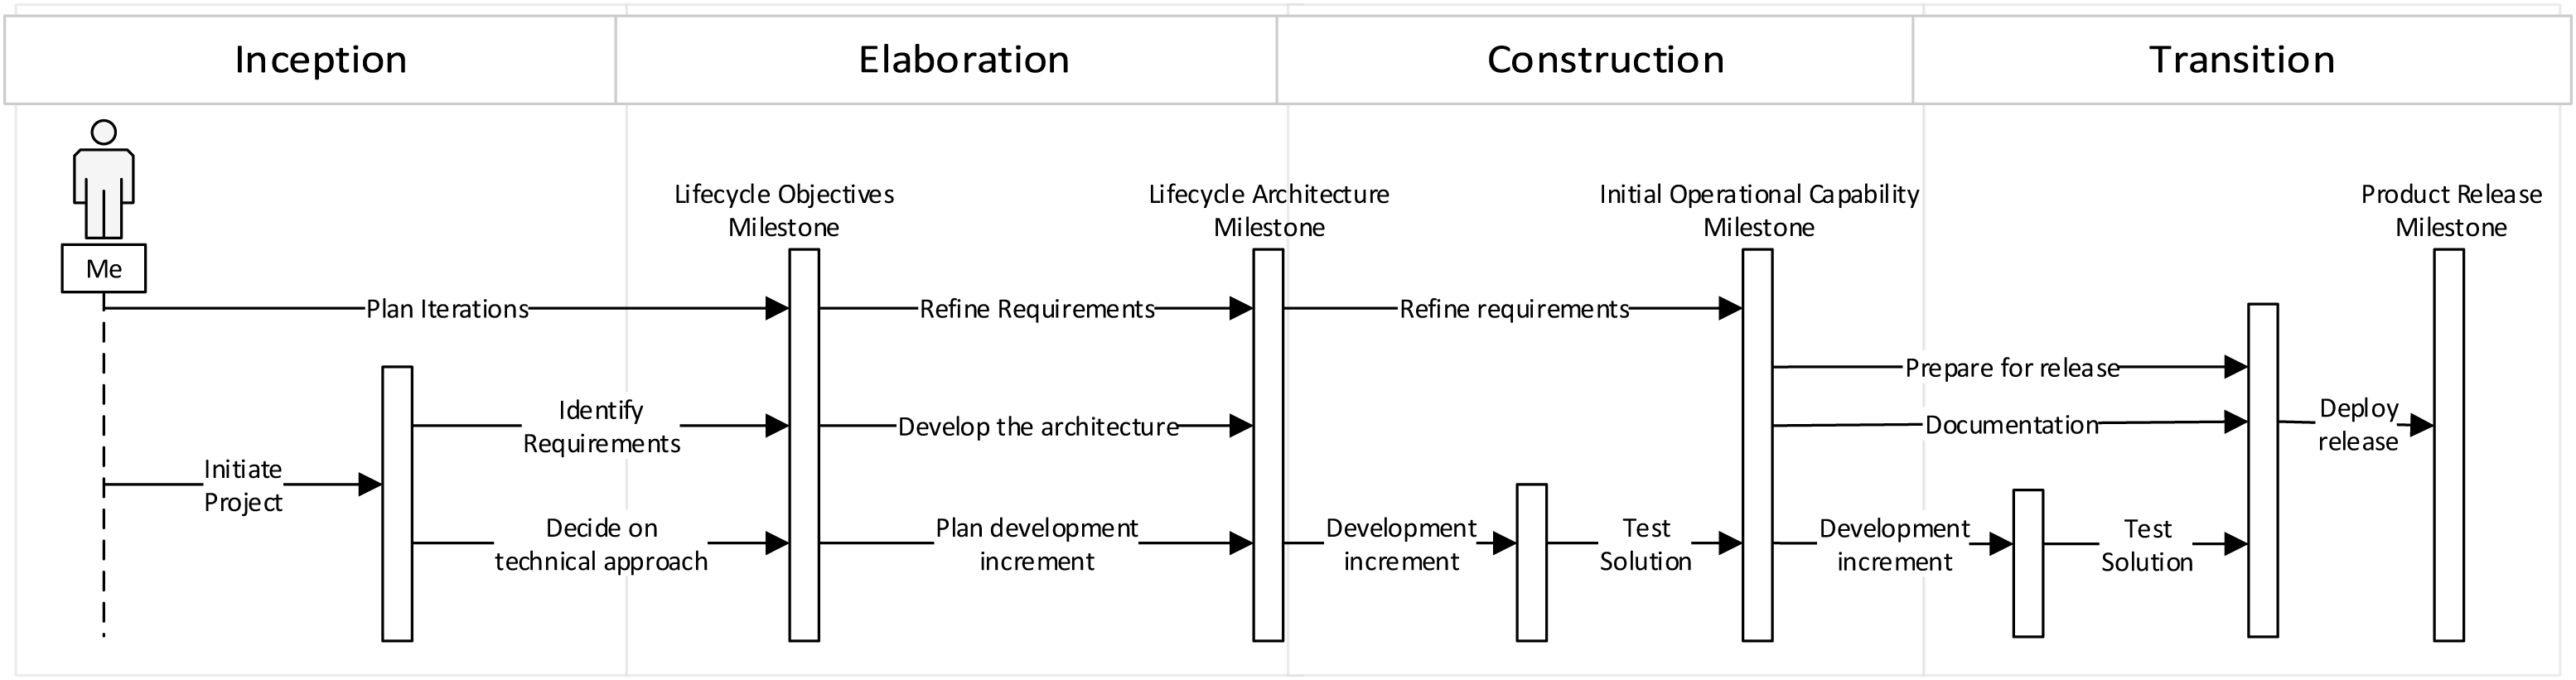
\includegraphics{assets/sequence-openup.png}
\caption{A sequence diagram showing a single full iteration of the OpenUP
  process}
\label{fig:graph-interval-dropped}
\end{figure}

\subsection{Work Breakdown Structure}
The crux of OpenUP is in breaking down a large development project into four key
phases to iterate on: the Inception Phase, Elaboration Phase, Construction Phase
and Transition Phase (7).

\paragraph{Inception Phase} The inception phase represents the initial work
which defines the scope and objectives of the project. Key tasks include
generating a list of the core project's requirements, key features and main
constraints, and developing an understanding of the general project use-cases
and business case. The work in this phase culminates with a stakeholder
concurrence on the project scope, cost and schedule, and a deep requirements
understanding which covers the depth and breadth of the technical work to be
undertaken. For this project, the inception phase should include meeting all
project stakeholders and research into existing protein databases, their
use-cases, and a deeper understanding of the scientific value of the dataset.

\paragraph{Elaboration Phase} The elaboration phase builds upon the work done in
the construction phase by requiring deeper technical research into required
technologies, and initial prototyping of early ideas. By the end of the
elaboration phase, the product vision should be agreed upon and stable, and a
full plan of the technical architecture should have been reached.  Further
iterations of the elaboration phase may be used after construction has begun to
refine the architecture plan, or as a response to a change in the technologies
used. The purpose of the phase is to turn the initial product vision into a
realisable goal with quantifiable and achievable goals and objectives. For this
project, the elaboration phase will involve investigation into some of the
available technologies (PHP, MySQL, Node.js, MongoDB, etc.), and technical
prototypes of the database backend.

\paragraph{Construction Phase} The construction phase covers the development of
the main software architecture and associated documentation, and should result
in ``Initial Operational Capability'' (7). Success criteria for this development
phase includes whether the product is mature enough to be deployed to users, and
so for this project will require meeting with stakeholders to ensure that the
implementation of the plan is acceptable.

\paragraph{Transition Phase} The transition phase includes beta testing of the
new system against user expectations, and includes a review of the completed
product against the requirements and objectives established in the initial
project plan to measure success. The phase culminates in a product roll-out and
the associated distribution, marketing and training of users that is
required. For this project, it will involve deploying the finished project to a
public server and conducting extensive user testing.

\subsection{Version Control}

A revision control and source code management (SCM) system will be used during
all development to keep an auditable and transparent log of progress, and Git
will be used for this. There are numerous advantages that Git has over other
SCMs, chiefly that it is entirely open source and GPL licensed (8), it has a
very lightweight branching model and good support for rebasing and merging, and
there are numerous sources which offer free hosting of open source licensed
projects that are tracked by Git. A public repository of the source code and all
relevant documentation for this project is available on GitHub (9).

\subsubsection{Issue Tracker}

One of the additional benefits of the GitHub online repository hosting service
is that it supplies a number of useful tools, namely an issue tracker and
milestones list. This allows issues to be created online and categorised
appropriately (e.g. bugs, tasks, regressions, documentation, etc.), and then
referenced from the repository commits.  Milestones can be created and
individual issues assigned to them, allowing for quick and visible progress
checking of development towards a specific goal.

\subsubsection{Test Driven Development}

\begin{figure}[H]
\centering
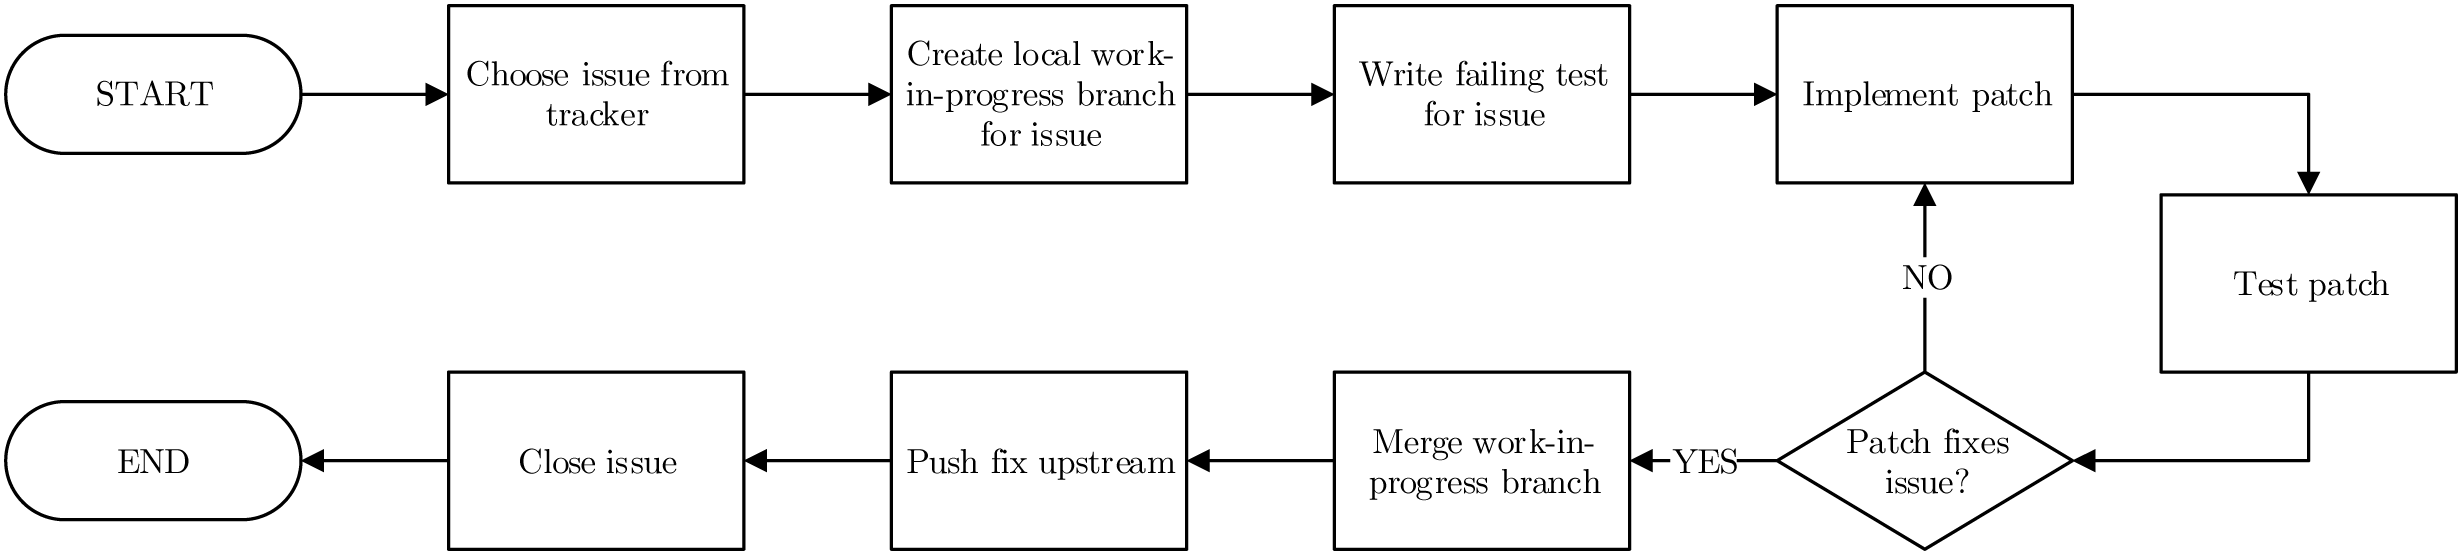
\includegraphics{assets/flow-tdd.png}
\caption{A single iteration of the project’s test-driven development workflow}
\label{fig:graph-interval-dropped}
\end{figure}

By combining the available issue tracker with good version control practises, it
is possible to implement a simple and functional test driven approach to
development (Figure 7). This breaks down the development process into
single-issue chunks, with each iteration beginning with creating a local
development branch for an issue and then writing failing test cases which can
then be patched. Using this model of development ensures that all work
undertaken is relevant to the project and directly affects progress, minimising
the amount of time wastage and increasing the stability of the codebase by
ensuring adequate test coverage (10).

\section{PROJECT SCHEDULE \hrulefill}
The project development is spread over a 26 week period, with 11 weeks in the
first teaching period and the remaining 15 in the second. In order to maximise
the effectiveness of this time, a list of tasks for each of the four OpenUP
development phases was constructed, and a time allowance associated with
each. The final project plan consists of 8 phases: the inception phase and
transition phases, and four iterations of elaboration and construction.  The
smaller elaboration and construction cycles were used so as to maximise the
allowance for changes in the project specification caused by user feedback and
review without causing delays in the development. This is to minimise the impact
of the ``Change in project requirements during development'' risk. Once the list
of tasks was assembled, a Gantt chart (page 16) was constructed which ordered
each of these tasks and distributed them across the timespan. Careful ordering
of the tasks ensured that there is the least chance for blocking between
activities, where one task runs over the specified time allowance and causes
later tasks to be postponed until it's finished.  The final project plan allows
for the maximum amount of parallel activities and development by ensuring that
there are adequate gaps between activities that depend on each other.

\subsection{Milestones}
In order to provide a running measure of success for the project, a set of
milestones were defined which track the development process from inception
through to transition and provides completion deadlines for a set of activities.
Two types of milestones are used: design and implementation.

Design milestones cover the design of the user interface, such as the ``look and
feel'' of the project, and the interaction design. Each design milestone is
preceded by a round of user testing, in which feedback and opinions can be
gathered by the project stakeholders in order to influence the next iteration of
design.

The implementation milestones cover the technical development, with each
milestone marking a set improvement in the implementation of the backend,
frontend, and controller, from the initial prototyping phase to the ``feature
complete'' endpoint. Unlike the design milestones, the implementation milestones
do not rely so heavily on input from third parties and so are more a personal
measure of my own development.

For each milestone, a set of requirements has been created which can be used as
success criteria for deciding when a milestone has been achieved. The
requirements of the milestones are cumulative, meaning that requirements for the
final milestone of each type includes all of the requirements of the previous
milestones of that type. In the case of the implementation milestones, the
requirements have been split into functional and non-functional requirements,
where functional requirements describe the behaviour and functionality of the
product, and non- functional requirements describe the criteria which can be
used to judge the functional behaviour.

\subsubsection{Design Milestones}

\paragraph{D1 First iteration design (week 3)} at this early stage of
development, the design should consist of a set of non-interactive ``paper
prototypes'' or static renders of the application interface, which can be used
as a rough guide for beginning to prototype the interaction design.

\begin{table}[H]
\centering
\begin{tabular}{ l l p{12cm} }
\textbf{ID} & \textbf{Type} & \textbf{Description}\\ \hline

D1.1 & Non-functional & A set of mock-ups for the design of common site pages:
search page, results page, details page (if applicable), advanced search, login
page, and upload new data page.\\

D1.2 & Non-functional & A set of interaction mock-ups for common site tasks:
searching for a record by protein name, searching records from a specific
source, searching for records in a pI range, performing an advanced search,
adding a new record, uploading a new dataset.\\

\hline
\end{tabular}
\caption{D1 milestone requirements}
\label{tab:d1-requirements}
\end{table}

\paragraph{D2 Second iteration design (week 13)} the user interaction design
should be the primary focus of this second iteration, with many of the common
tasks (searching for a result, looking up a record, etc.) being more tightly
defined.

\begin{table}[H]
\centering
\begin{tabular}{ l l p{12cm} }
\textbf{ID} & \textbf{Type} & \textbf{Description}\\ \hline

D2.1 & Functional & An interactive prototype which implements common site tasks:
logging in and out using credentials, searching for a record by protein name,
searching records from a specific source, searching for records in a pI range,
performing an advanced search, adding a new record, uploading a new dataset.\\

D2.2 & Non-functional & A set of interaction mock-ups for ‘edge case’ or
uncommon events: an error on the server-side, performing a search which returns
no results, attempting to log in with incorrect credentials.\\

\hline
\end{tabular}
\caption{D2 milestone requirements}
\label{tab:d2-requirements}
\end{table}

\paragraph{D3 Third iteration design (week 18)} by the third iteration, the
interaction design should be complete, allowing the focus of development to be
placed on polishing the look and feel of the application and establishing a
common aesthetic style.

\begin{table}[H]
\centering
\begin{tabular}{ l l p{12cm} }
\textbf{ID} & \textbf{Type} & \textbf{Description}\\ \hline

D3.1 & Functional & An interactive website which implements the full interaction
design.\\

D3.2 & Non-Functional & A set of revised mock-ups for the aesthetic design of
all site pages.\\

\hline
\end{tabular}
\caption{D3 milestone requirements}
\label{tab:d3-requirements}
\end{table}

\paragraph{D4 Finalised design (week 24)} this last design milestone marks the
endpoint of all design changes, and can be used to review the quality and
effectiveness of the fully evolved product.

\begin{table}[H]
\centering
\begin{tabular}{ l l p{12cm} }
\textbf{ID} & \textbf{Type} & \textbf{Description}\\ \hline

D4.1 & Functional & An interactive website which implements the full aesthetics
and interaction design, providing 100\% coverage of all interactions and
scenarios described by the mock-ups.\\

\hline
\end{tabular}
\caption{D4 milestone requirements}
\label{tab:d4-requirements}
\end{table}

\subsubsection{Implementation Milestones}

\paragraph{M1 Initial prototype (week 11)} by the end of the first term,
breath-first and depth-first prototypes of the system which some of the more
common user tasks should have been implemented, although the underlying software
architecture and technologies are free to change for the production system.

\begin{table}[H]
\centering
\begin{tabular}{ l l p{12cm} }
\textbf{ID} & \textbf{Type} & \textbf{Description}\\ \hline

M1.1 & Functional & A breadth-first prototype which implements coverage for the
common site pages and tasks.\\

M1.2 & Functional & A depth-first prototype of the user accounts system and data
back-end.\\

M1.3 & Functional & The prototype should allow for potential users to interact
with a website which implements a limited subset of the final functionality,
allowing for early feedback on the design.\\

M1.4 & Non-Functional & An architectural design for the final system database.\\

M1.5 & Non-Functional & A tool to generate fake datasets and upload them to the
prototype for testing purposes.\\

\hline
\end{tabular}
\caption{M1 milestone requirements}
\label{tab:m1-requirements}
\end{table}

\paragraph{M2 Working system (week 18)} by week 18 the software architecture and
choice of technologies should have been fully realised, and the functional
backend of the majority of use-cases should have been implemented, along with
good test coverage of each.

\begin{table}[H]
\centering
\begin{tabular}{ l l p{12cm} }
\textbf{ID} & \textbf{Type} & \textbf{Description}\\ \hline

M2.1 & Non-Functional & A software design which stipulates the final decision on
which technologies will be used.\\

M2.2 & Non-Functional & An architectural design which covers the full model view
controller stack and components of each.\\

M2.3 & Non-Functional & A test harness and accompanying automated unit tests
with full coverage of the API under common states.\\

\hline
\end{tabular}
\caption{M2 milestone requirements}
\label{tab:m2-requirements}
\end{table}

\paragraph{M3 Feature complete (week 24)} the feature complete milestone marks
the end of the development of new features. By this point, the system should be
fully functional and optimised, allowing for final stress and load testing to
take place, and for the system to be deployed.

\begin{table}[H]
\centering
\begin{tabular}{ l l p{12cm} }
\textbf{ID} & \textbf{Type} & \textbf{Description}\\ \hline

M3.1 & Functional & A secured server which is publicly accessible from a domain
name.\\

M3.2 & Functional & An optimised software stack which can serve pages within a
determined time limit.\\

M3.3 & Functional & A software architecture which can support datasets of up to
a million records.\\

M3.4 & Non-Functional & Full test coverage of the API and automated black-box
testing of the common website tasks.\\

M3.5 & Non-Functional & The source code should be available online and licensed
with an appropriate open source license.\\

M3.6 & Non-Functional & Full documentation coverage of the internal API.\\

\hline
\end{tabular}
\caption{M3 milestone requirements}
\label{tab:m3-requirements}
\end{table}

\newpage
\section{Project Gantt Chart}
\label{appendix:project-gantt-chart}

\begin{figure}[H]
\centering
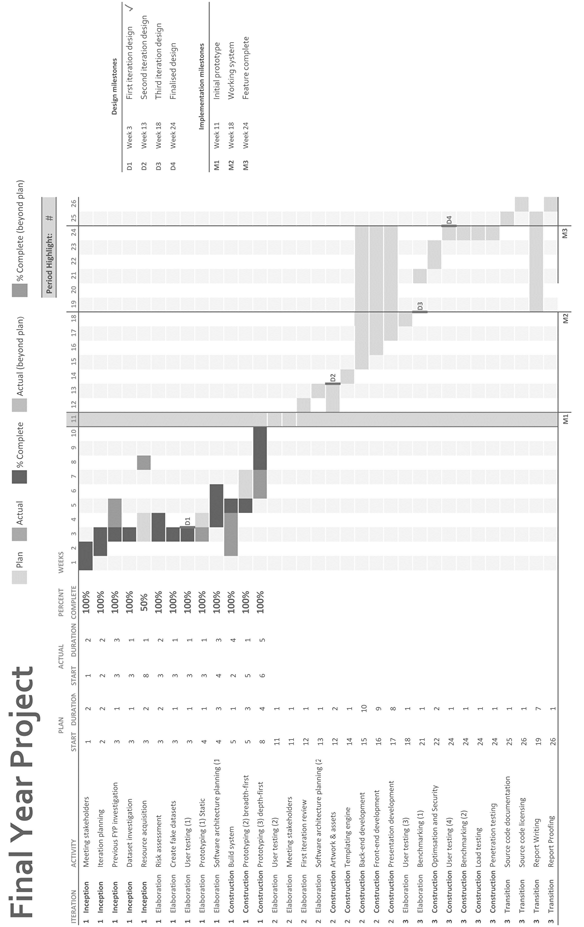
\includegraphics{assets/gantt-plan.png}
\end{figure}

\newpage
\section{Previous Final Year Project Database Design}
\label{appendix:previous-fyp-uml}

\begin{figure}[H]
\centering
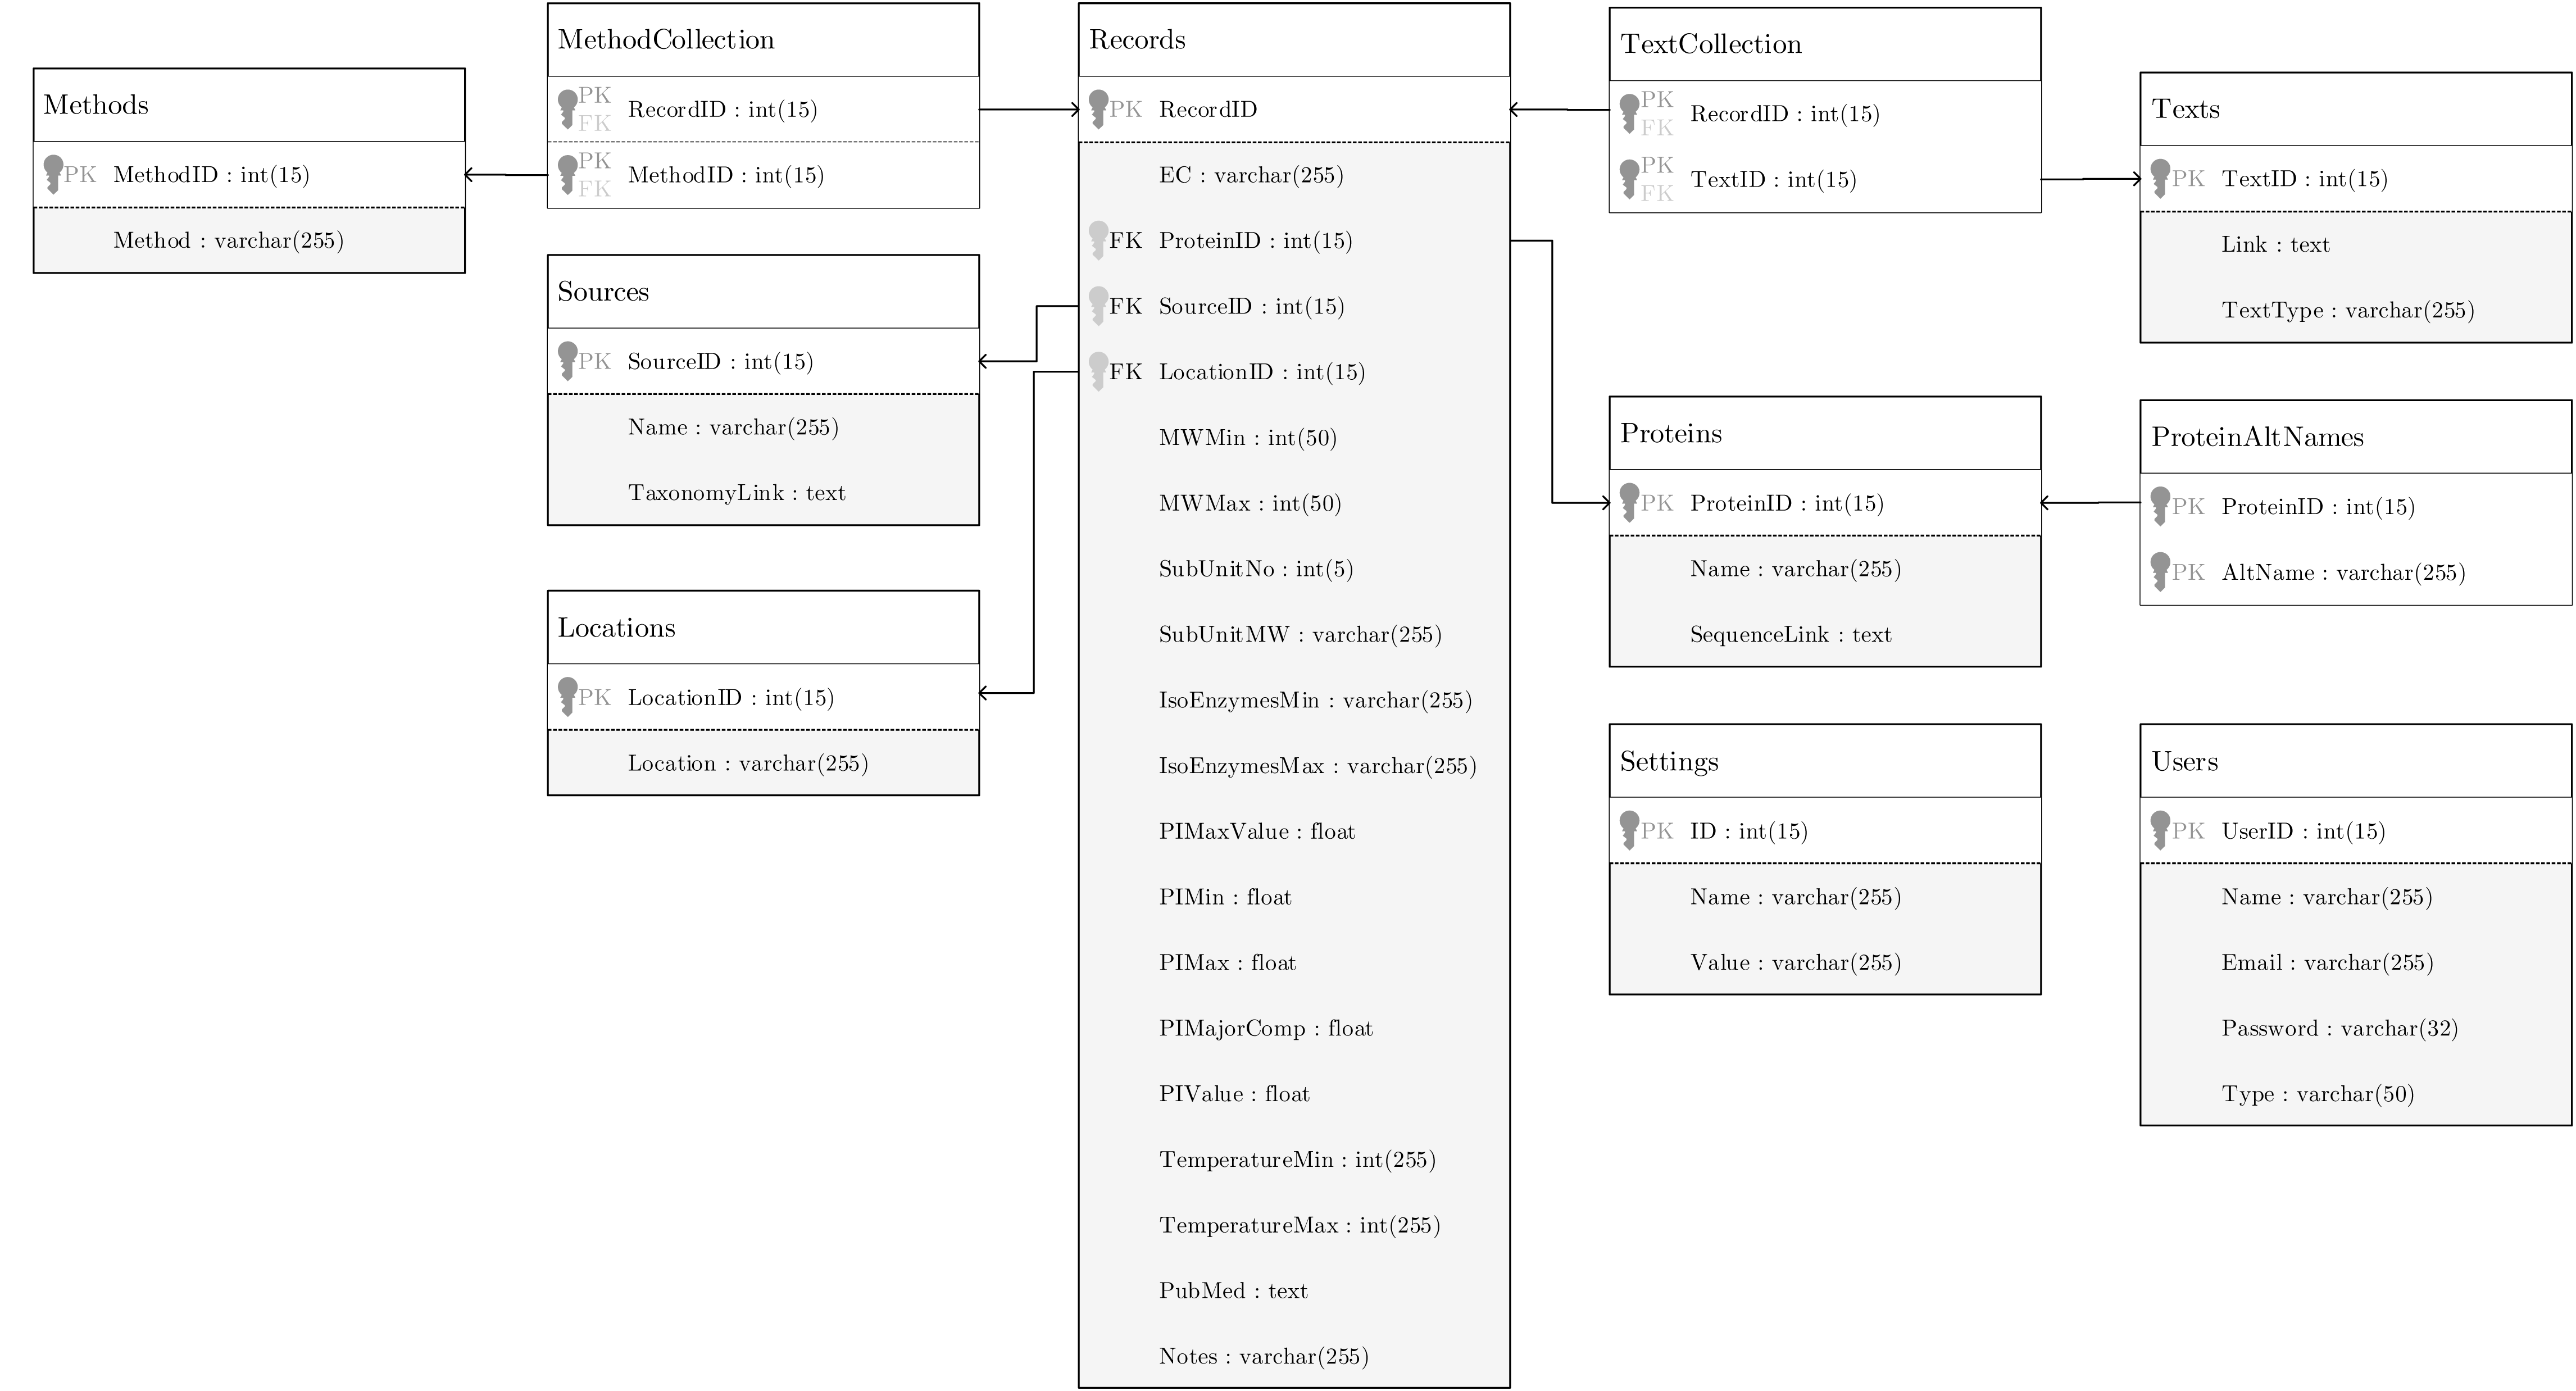
\includegraphics{assets/uml-previous-fyp-database.png}
\end{figure}

\newpage
\appendix
\setcounter{secnumdepth}{1}
\begin{subappendices}

\end{subappendices}

\newpage
\begin{thebibliography}{9}

\end{thebibliography}

\end{document}
